\chapter{Approach for Solving the Issue} \label{approach}
% DELETEME: In this chapter you start addressing your actual problem. Therefore, it makes often sense to make a detailed problem analysis first (if not done in introduction). You should be sure about what to do and how. While writing in the background part, it might also make sense to include complex background information or papers you are basing on in this analysis. If you are solving a software problem, you should follow the state of the art of software development which basically includes: problem analysis, design, implementation, testing, and deployment. Maintenance is often also described but I believe this will not be required for most theses. Code should be placed in the appendix unless it is solving an essential aspect of your work.

This chapter provides an explanation of what techniques were used in the problem's solution. It is split into smaller subsections, which consider different parts of the proposed strategy.

\section{Organisation of the Simulation}
In general, to conduct real-world experiments is rather expensive and time-consuming, therefore we simulate different scenarios using CARLA. What is more, there are no limitations in the digital environment and data samples can be created faster without any distortions or noise. It offers an opportunity to implement and test different approaches and ideas in ideal conditions where no real-life restrictions exist.

Our simulation takes place in a realistic digital city "Town10HD\_Opt" from the CARLA assets package, which represents a whole town including, i.e., buildings, trees, traffic lights, parked vehicles, etc. The main location of the experiments is a junction of four roads, because, compared to other types of intersections, there exists a higher chance for accidents to happen, and an optimal camera placement is crucial for a safe mobility. On the junction's premises we place 3 CARLA objects from type Actor: 
\begin{itemize}
    \item 1 camera and 2 vehicles, which has the roles 'occluder' and 'target'
\end{itemize}
In pursuance of finding an optimal position for the camera sensor we consider the 4 angles of the region of interest (ROI) and also the points in the middle of each of the 4 edges like it is shown in Figure \ref{fig:camera_positions}. In this way, we earn an approximate idea which point or area has to be aimed for when placing a camera. Furthermore, this placement could be applied to other infrastructure of the same type, therefore it also guarantees flexibility and universality of the approach. 

With regard to the vehicles, which play the most important role in our research, we divide them into two categories:

\begin{itemize}
    \item \textbf{Occluder vehicle} - stays between the sensor and the target vehicle and covers some part of it because of its larger size or position regarding the sensor. For a realistic scenario we use a medium and large-sized vans or trucks, so that their shape generate a blind zone for the sensor's field of view, which then cannot recognize the occluded vehicle. 
    \item \textbf{Target vehicle} - is equal or smaller than the occluder, because we have to measure the degree to which it is occluded in various positions. If, for example, it has the bigger proportions, the chance of a camera not detecting it is quite decreased even if it stays behind the occluder. 
\end{itemize}
During the simulation we spawn both vehicles in different locations on the intersection in order to reproduce as many as possible dynamic situations and decide whether an occlusion occurs or not.

\begin{figure} [h]
    \centering
    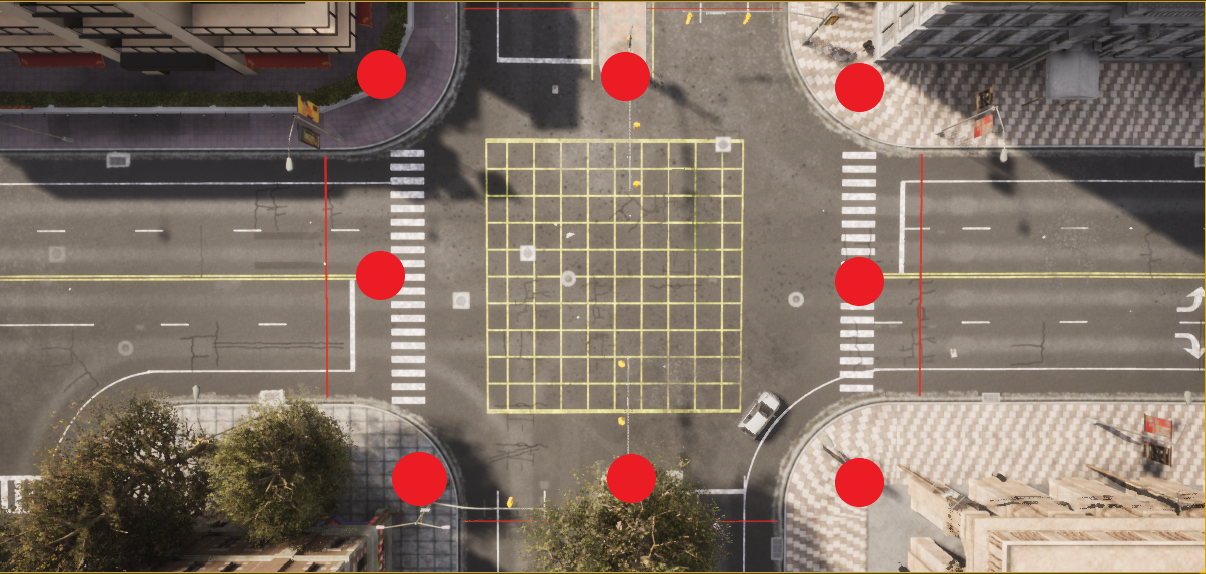
\includegraphics[width=\textwidth]{images/junction.png}
    \caption[Camera experiment positions]{This picture displays an example where the camera is going to be placed during simulations and shows the borders of our region of interest.}
    \label{fig:camera_positions}
\end{figure}

\section{Simulation Pipeline} \label{sec:sim_pipeline}

This thesis relies on a simulation pipeline for conducting experiments and evaluating their output, which consists of three main stages that can be seen on Figure \ref{fig:evaluation_pipeline}: 

\begin{enumerate}
    \item \textbf{Preparation of the experiment} - encompasses the configuration of all virtual world settings, as well as the creation of points on the test intersection that will be used during the experiments. In this stage a camera object is spawned within the simulated environment, which perceives the traffic and returns data that has to be evaluated. 
    \item \textbf{Reproduction of possible scenarios} - during this stage we have tuples of vehicles(occluder and target) that are spawned on the waypoints generated in the previous stage. In addition, after each new spawn, images from the camera are saved for further evaluation of the occlusion degree and the other metrics.
    \item \textbf{Evaluation of results} - being the last stage of the simulation pipeline, here the results are evaluated and used to generate a heatmap and a graph for a better visualisation, after which we discuss in \ref{evaluation} how our approach optimises traffic camera placement.
\end{enumerate}
In the following subsections we provide a more detailed explanation of how all the process from data generation via vehicles placement to output evaluation is realised.
\begin{figure} [h]
    \centering
    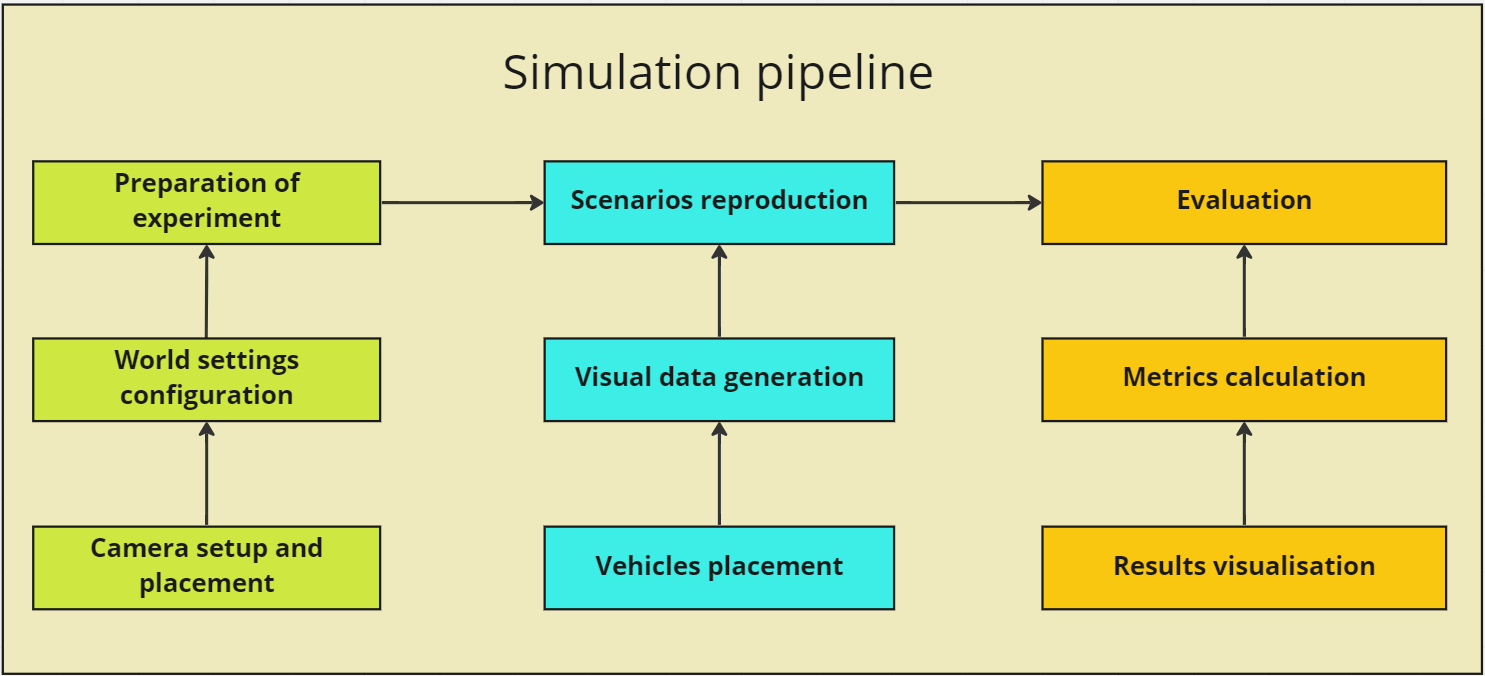
\includegraphics[width=\textwidth]{images/evaluation_pipeline.png}
    \caption[Evaluation pipeline]{This diagram represents schematically the simulation pipeline}
    \label{fig:evaluation_pipeline}
\end{figure}

\subsection{Experiment Setup and Environment Preparation}
As a prerequisite for each simulation it is important to adjust the world settings correctly in order to maintain a synchronous mode, which allows for reliable data from the sensors. In CARLA we set a client which communicates with our world and a traffic manager which is responsible for the behaviour of vehicles. 

When we are done with the creation of our simulated environment, the main priority is to generate waypoints within the intersection, which serve as spawn points for the vehicle actors. To clarify, all points belong to the road, where cars usually drive and no cases where a car spawns on the pavement or on a green area are considered. Furthermore, each point defines apart from the location also the direction in which the vehicle's head will point, therefore no situations like a car in the opposite direction or perpendicular to both driving directions occur in the experiments. For the purpose of covering maximal number of occlusion situations on the road we collect each existing waypoint in Figure \ref{fig:waypoints} that the simulator offers between the borders of the junction. On Figure \ref{fig:camera_positions} the ROI, defined by red borderlines, can be seen.

At the end of the preparation step we spawn a camera actor which should monitor all scenarios and perceive crucial for the research data. Therefore, cameras are positioned on such points, where they achieve maximal coverage of the region of interest and are able to avoid more potential occlusions. Each camera have adjustable parameter that are described in Table \ref{tab:camera_params}. In addition to these parameters, we define the camera tilt angle in a vertical plane, whose degree value is such that the camera field of view covers a bigger part of the intersection. 
\begin{table}[h]
\caption{Table for camera parameters and definitions used in this thesis\label{tab:camera_params}}
\centering
    \begin{tabular}{ | l | p{5cm} |}
    \hline
    Parameter & Definition  \\ \hline
    fov & Horizontal field of view in degrees. \\ \hline
    image\_size\_x & Image width in pixels. \\ \hline
    image\_size\_y & Image height in pixels. \\ \hline
    \end{tabular}
\end{table}

\begin{figure} [h!]
    \centering
    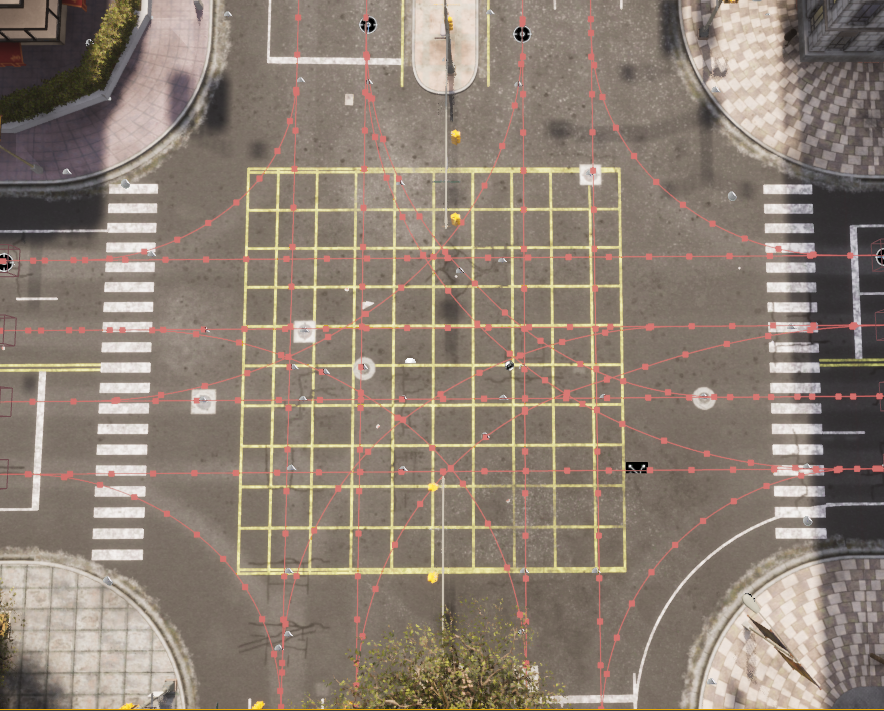
\includegraphics[width=0.7\textwidth]{images/waypoints.png}
    \caption[Intersection waypoints]{This picture illustrates all available spawn points for our vehicles}
    \label{fig:waypoints}
\end{figure}
\newpage

\subsection{Simulation of scenarios} \label{sec:sim_stage}
One main problem is that most of the researches considers only static obstacles as occluder when executing their experiments and do not take into account the dynamic occlusion. Therefore, we follow the idea of \cite{occlusion_degree_model} and apply a similar approach in our work. Like mentioned in \ref{sec:sim_pipeline} we use vehicles as actors for our experiments, which we spawn on previously generated waypoints. The idea of this strategy is to have two different by size vehicles, which are called an 'occluder' and a 'target', because we aim to reproduce the occlusion that happens each day in traffic. Autonomous vehicles require an accurate perception of the world around them to avoid accidents, which is why we recreate various scenarios by placing the vehicles on each pair of points. By doing so, we get the chance to analyse dynamic occlusion without the need of moving objects.

Vehicles in this work could not be placed on the same spawn point simultaneously and also positions, not included on the image plane, are not examined. Furthermore, depending on the waypoint there could be several directions for the vehicle, which also has impact on the volume of the blind zone caused by the larger vehicle. 

Due to the focus being on the occlusion degree, we have to know what percentage of the target vehicle is occluded. One way to overcome these problems is to use the bounding boxes of each vehicle, which are provided by the simulator. Our first idea was to convert all its eight vertices from the 3D world to the 2D image plane by choosing the upper-, lower-,  left- and rightmost points as exemplified with red points in Figure \ref{fig:bb_conversion}. Subsequently, we have an approximate 2D representation of the vehicle's borders and can subtract the visible part from the occluded car. However, after some experimentation with this strategy, it was asserted that this method is inefficient and unreliable. In comparison to the following approach, this one returns results with ca. 30-40\% difference from the correct and expected values. The main reason that justifies this behaviour is that a bounding box contains more points or pixels than these, which belong to the vehicle. Therefore, we needed another solution that calculates the occlusion precisely, which would be of utmost importance if later our approach is applied in a real-world scenario.
In our current implementation, due to the lack of depth information from a normal monocular camera, an instance segmentation camera (see \ref{instance_camera}) is applied instead of using an algorithm for object detection. The main advantages compared to previous method are mainly simplicity and accuracy, because this camera type provides us with ground-truth data in the form of an image, whose pixels have colour values according to the object each of them contain. It works like a 100\% accurate algorithm for object recognition, therefore it should be taken into account if the strategy is adopted by future works that depth information is a prerequisite for a reliable real-world implementation.

In order to calculate the correct percentage of occlusion, first is spawned the target vehicle, its number of pixels on the image plane are counted (see implementation in \ref{subsec:calc_occl}) and then the occluder is spawned. When both vehicles are present in the world, we can extract the part under occlusion. However, it is possible that in particular cases no occlusion exists, i.e., when the occluder is not positioned between the sensor and the target vehicle. In Figure \ref{fig:occlusion_views} it is shown how depending on the point of view an occlusion is either visible or does not occur. After each tuple of points is observed the implementation returns the following output, which is saved in a text file:
\begin{itemize}
    \item world coordinates of target vehicle (x, y, z)
    \item rotation of target vehicle (pitch, yaw, roll)
    \item occlusion degree given in percent
\end{itemize}

\begin{figure} [h!]
    \centering
    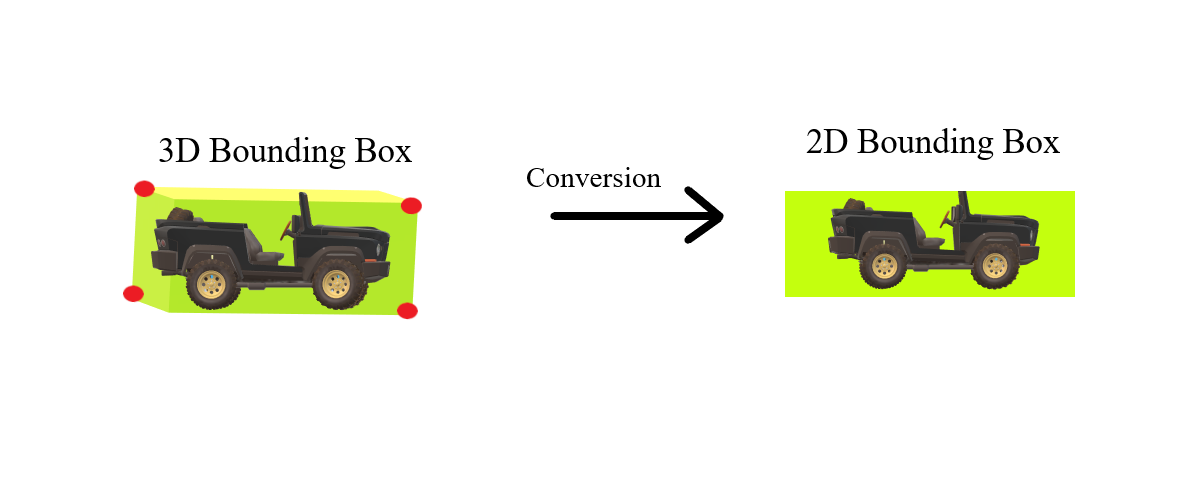
\includegraphics[width=0.8\textwidth]{images/2D_bounding_boxes.png}
    \caption[3D bounding box conversion]{On this illustration is shown the conversion from a 3D bounding box to a 2D one, which a camera would perceive.}
    \label{fig:bb_conversion}
\end{figure}

\begin{figure} [h!]
  \centering
  \subfloat[Occlusion from camera's point of view]{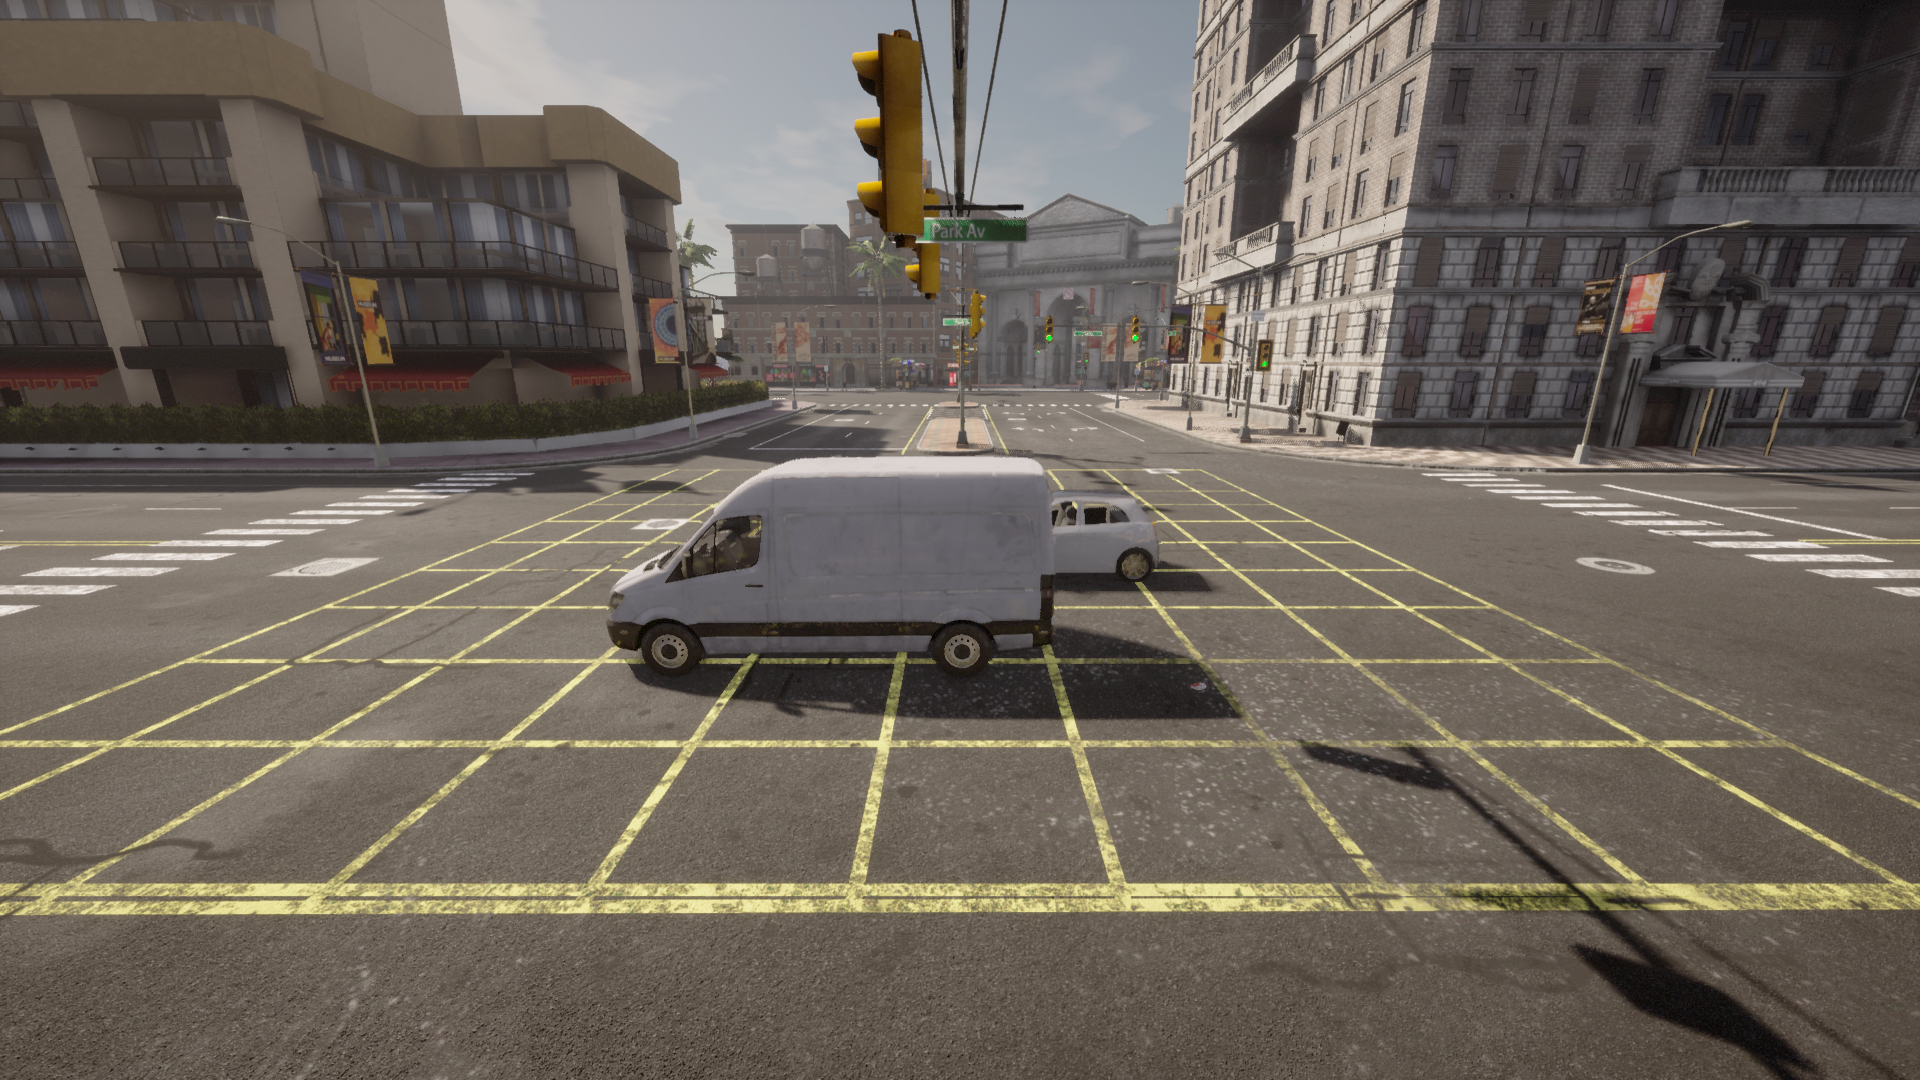
\includegraphics[width=0.574\textwidth]{images/camera_view_occlusion.jpg}}
  \hfill
  \subfloat[Occlusion from side point of view]{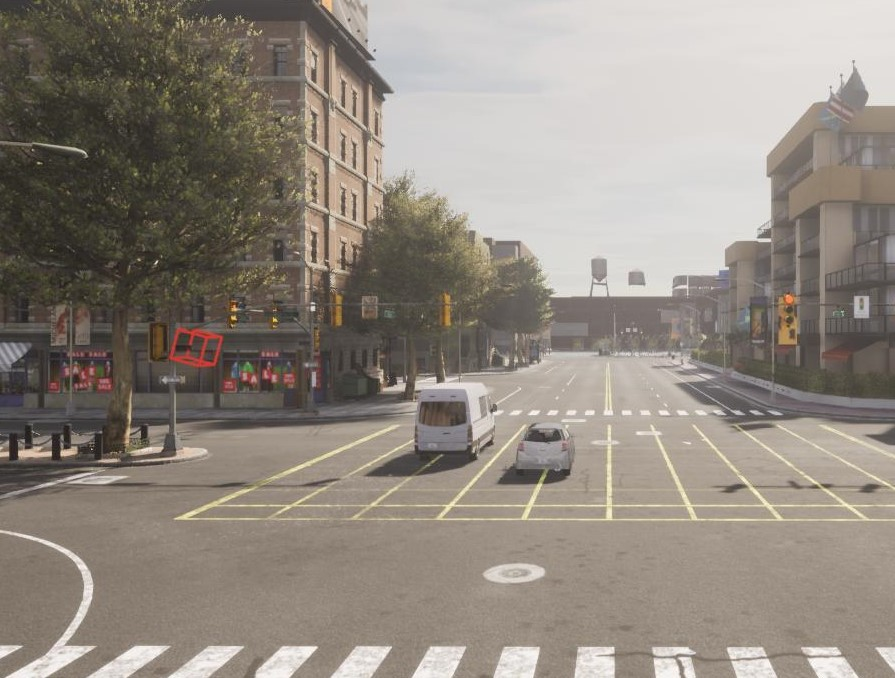
\includegraphics[width=0.426\textwidth]{images/different_view_occlusion.jpg}}
  \caption[Occlusion points of view]{These two images display how an occlusion is perceived from different points of view.} \label{fig:occlusion_views}
\end{figure}

\newpage
\subsection{Evaluation of Results}
When we already have the data from the simulation stage, it should be visualised for a better understanding of the results. In the evaluation stage, this thesis makes use of heatmap to illustrate where the occlusion occurs at most and thus choose the most optimal point of view for a camera. For the purpose of a coherent visualisation we discretise the intersection in equal rectangular blocks where each block has world X and Y coordinate values. Furthermore, to each of these blocks are assigned the positions where the target vehicle has been spawned. As mentioned in \ref{sec:sim_stage}, we receive an occlusion degree for each tuple of the junction's waypoints, which means that for a single position of the target we usually have more than one occlusion degree available. For this reason, during the generation of a heatmap for each saved spawn position in the result file, we calculate the average occlusion from all the values assigned to the position and display it on the map with an according colour from the colour palette. We use the heatmaps to explain whether the camera placement is optimal or not according to the amount of occlusion it detects, i.e., light colours imply that a little amount of occlusion was perceived whereas darker colours indicate loss of sight and an unfavourable sensor position.

In addition to the occlusion degree, we also rely on two metrics, which are inspired by \cite{occlusion_degree_model}, when comparing the performance of cameras placed on different locations. The first one estimates the ratio of times a target vehicle on a specific position is not detected by a camera because the occlusion percentage exceeds the particular threshold for object recognition to all times it has been on this location. Our second metric is the ratio of vehicles missed by the sensor in case they are out of its field of view to the total amount of traffic. When these two metrics have lower values, we are able to determine where is a reasonable area for camera installation, which will ensure a better traffic surveillance. 
